\documentclass[letterpaper,doc,natbib]{apa6}

\usepackage{setspace}
\doublespacing

\usepackage[english]{babel}
\usepackage[utf8x]{inputenc}
\usepackage{amsmath}
\usepackage{graphicx}
\usepackage[colorinlistoftodos]{todonotes}
\usepackage{amssymb}

\title{Realistic Textures of Surface Weathering using\\
Generative Adversarial Networks}
\shorttitle{ }

\author{Budmonde Duinkharjav\\
{\tt\small budmonde@mit.edu}
}
\affiliation{Advised by Prof. Fredo Durand, CSAIL Computer Graphics Group\\
M.Eng Thesis Proposal, Fall 2018\\
Massachusetts Institute of Technology
}

\begin{document}
\maketitle

\section{Introduction}

Recent advances in computer vision research have presented impressive results in its ability to generate high fidelity procedural textures. Despite the visually appealing results, recent models rely heavily on the existence of high-quality exemplars to learn textures from. This requirement limits the application of existing models such as learning the texture of weathering on a car (dirt, rust, and scratches), from natural images of weathered cars. Creating a model that learns complex textures from natural images could be useful in computer graphics, enabling us to build mode photorealistic graphics simulations.

In this thesis, we propose a model for using images of weathered cars to learn a texture that could be readily applied to a 3D car mesh which would simulate the weathering of the material.

This project is part of a larger overarching project Toyotacity, led by Prof. Fredo Durand, which attempts to generate procedurally generated city streets with cars, pedestrians, traffic lights, etc. Being able to create a synthetic dataset with configurable knobs which control different parameters of the city such as the diversity of the cars, the number of pedestrians, time of day etc. is critical as it allows for systematic studies of different computer vision models and their performances in varying circumstances.

\section{Related Work}

Generative Adversarial Networks (GANs) framework introduced by \cite{gan} has been proven to be a powerful framework for generating high fidelity images in the computer vision literature \cite{pix2pix}, \cite{cyclegan}, \cite{texsyn}, etc. However, GANs require the generator to be a differentiable function with respect to input variables. This means that when it comes to very complicated procedures such as ray tracing, calculating a derivative becomes a very difficult task. Fortunately, with the recent advent of the Differentiable Monte Carlo Ray Tracer by \cite{dmc}, we are able to apply adversarial training into the realm of computer graphics.

Similar to their paper, we define $R$ as a differentiable ray tracer which takes, as input, the scene description (camera pose, scene geometry, materials and lights) and outputs an image of the scene. If we perturb one variable from the scene description such as the position of the camera or a single pixel value from the material image, we will observe a change in the rendered image. Conceptually, since we can vary the input variables smoothly to observe a smooth change in the rendered image, we should be able to calculate the partial derivative with respect to some scene variable $x$ of the render function $R$ while keeping all other scene variables $\theta$ constant. The differentiable ray tracer provides a method for tractably calculating these partial derivatives as shown in Equation \ref{eqn:dmc}.

\begin{equation} \label{eqn:dmc}
\begin{split}
    y' & = R(x; \theta)\\
    \frac{\partial y'}{\partial x} & = \frac{\partial R(x; \theta)}{\partial x}
\end{split}
\end{equation}

\section{Formulation}
Our task is as follows: given an object (e.g. a car), its 3D mesh $M$, and a set of real images $Y$ depicting the object, we want to learn a texture-map $x \in X$ which when applied on $M$ and rendered using a Monte Carlo Ray Tracer $R : (\Phi, M, X)  \rightarrow Y'$ ($\Phi$ is the scene parameter set including camera pose, scene geometry and lighting parameters), produces a result $y' \in Y'$ that is indistinguishable from a real image. I.e. $y' \in Y$.

\begin{figure}
\centering
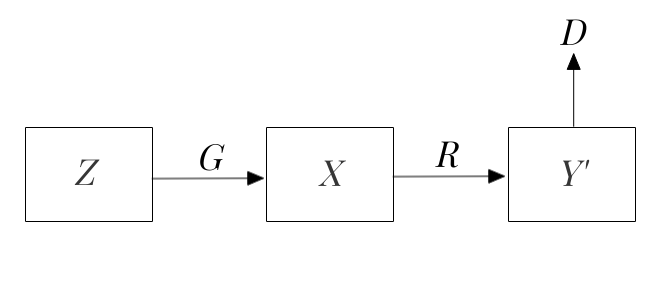
\includegraphics[width=0.7\textwidth]{formulation.png}
\caption{\label{fig:formulation} Our model contains a texture-map generation function $G : Z \rightarrow X$, a differentiable ray tracing function $R$ and a discriminating function $D$, which distinguishes natural images from generated images produced by the combination of $G$ and $R$.}
\end{figure}

Following the GAN framework, we learn a generator $G : Z \rightarrow X$ which produces some texture-map from a latent noise vector $z \in Z$, along with a discriminator $D$ which distinguishes images in the set of real images $Y$ from the set of rendered images $Y' = \{R(G(z); \Phi, M)\}$. Our objective is then to match the distributions of $Y$ and $Y'$ by minimizing the adversarial loss defined as:

\begin{equation} \label{eqn:advloss}
    \mathcal{L}_{GAN}(G, D) = \mathbb{E}_{y \sim p_{data}(y)} [\log D(y)] + \mathbb{E}_{z \sim p_{data}(z)} [\log (1 - D(R(G(z); \Phi, M)))].
\end{equation}

Equation \ref{eqn:advloss} is similar to the standard formulation of a GAN \cite{gan}. The only notable exception is that we're taking advantage of the Differentiable Monte Carlo Ray Tracer (\cite{dmc}) which allows us to use gradient descent with this loss function.

\section{Methods}

We adopt the network architecture from \cite{resnet} as our baseline model. The ResNet generator architecture has proven to be effective and stable as shown by \cite{cyclegan} and \cite{texsyn}.

Due to the intrinsic difficulty in training GANs (\cite{ganhard}), we have elected to make incremental improvements in order to reach our final goal of generating a model for texture generation of car surface weathering. Below we will list the steps we shall take to reach our final goal:

\subsection{1. Learning a texture from a simple plane}

The processs of rendering a 3D car mesh consists of painting a large number of triangles with a specific texture that is stored on an image. The scene would also contain information of the mapping between each triangle in the mesh and the texture coordinates that correspond to it (this concept is called UV-mapping in the literature). To simplify the problem, we could replace the thousands of triangles used for the car mesh into a square plane which consists of only two triangles as shown in Figure \ref{fig:perspective}. We would apply a texture on the two triangles and attempt to render it using the ray tracer.

In this setup, we pick a target texture we'd like to learn and render a scene using the target texture. Then, we'd want to train our model to be able to learn the target texture using only the rendered images of the target texture.

Our first benchmark for the project would be to train a model that successfully learns the target texture. Reaching this benchmark would provide us insight on the feasability of being able to train a model with a ray tracing step in it. We could further check the robustness of the model by changing the camera pose in the scene such that we would be looking at the plane at a slant (as shown in Figure \ref{fig:perspective}). If we are able to observe foreshortening in the generated images, we can conclude that the system is behaving as expected.

\begin{figure}
\centering
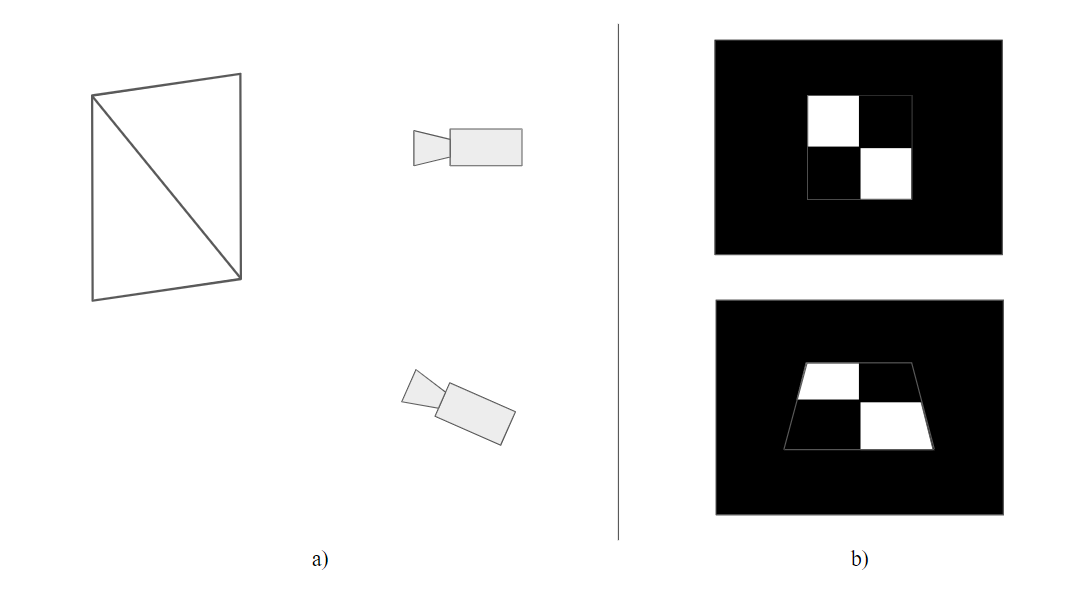
\includegraphics[width=0.95\textwidth]{perspective.png}
\caption{\label{fig:perspective} (a) The simplified experimental setup for incorporating a ray-tracing step in the learning process features a scene that with two triangles used to represent a flat plane. This plane is rendered from different angles to simulate a foreshortening effect (b) that allows graphical systems to simulate depth perception.}
\end{figure}

\subsection{2. Splitting the texture into separate layers}

In many graphical systems, texture "add-ons" such as weathering and dirt are applied separately to the base material a mesh could consist of. For example, if we have a table rendered with a wooden texture and we want the table to look dirty, rather than generating a whole new texture for "dirty wood", we would instead generate a semi-transparent dirt texture which would layer on top of the wooden texture as shown in Figure \ref{fig:layers}. This way, we separate the base material of the geometry from the weathering that could be applied to it. Separating the main task of learning weathering textures from different instances of similar materials helps us to isolate our task from other variables within the scene.

\begin{figure}
\centering
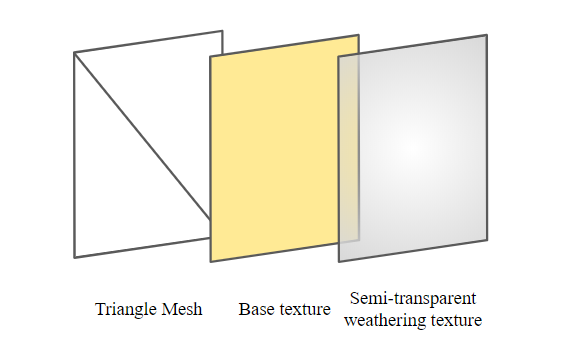
\includegraphics[width=0.7\textwidth]{layers.png}
\caption{\label{fig:layers} Base material in yellow is separate from the semi-transparent weathering material. Separating the two materials allows the model to only learn the weathering material while ignoring the diversity in base materials across learning examples.}
\end{figure}

In addition we would want to add more features to the texture-map such as a normal map. Normal maps give textures a non-flat three dimensional look. The normal map is a 3-channel image with each channel representing the different dimensions of the normal vector at any point on the texture map. This normal map is used by the ray tracer to simulate the non-flatness of a texture.

\subsection{3. Applying the model to a car mesh and training on a simulated dataset}

With the model tested for basic robustness in the prior steps, the next steps would be to render the mesh with a specular texture to simulate a clean car, and layer it with a semi-transparent weathering texture as described in the previous step. In order to simplify the UV-mapping from coordinate space to texture-space we shall use a spherical coordinate system with an origin at the bottom center of the car as shown in Figure \ref{fig:coordinates}.

To describe how this mapping would work let's consider a point $p$ on the surface of the car. In the spherical coordinate system, the point $p$ would correspond to coordinates $(r, \phi, \theta)$ where $r$ is the radius from the origin, $\phi$ is the azimuthal angle and $\theta$ is the polar angle respectively. Then we could have the point $p$ in coordinate space correspond to the azimuthal projection coordinates on the texture map at coordinates $\phi, \theta)$. This correspondence is shown in Figure \ref{fig:coordinates} for further clarity.

\begin{figure}
\centering
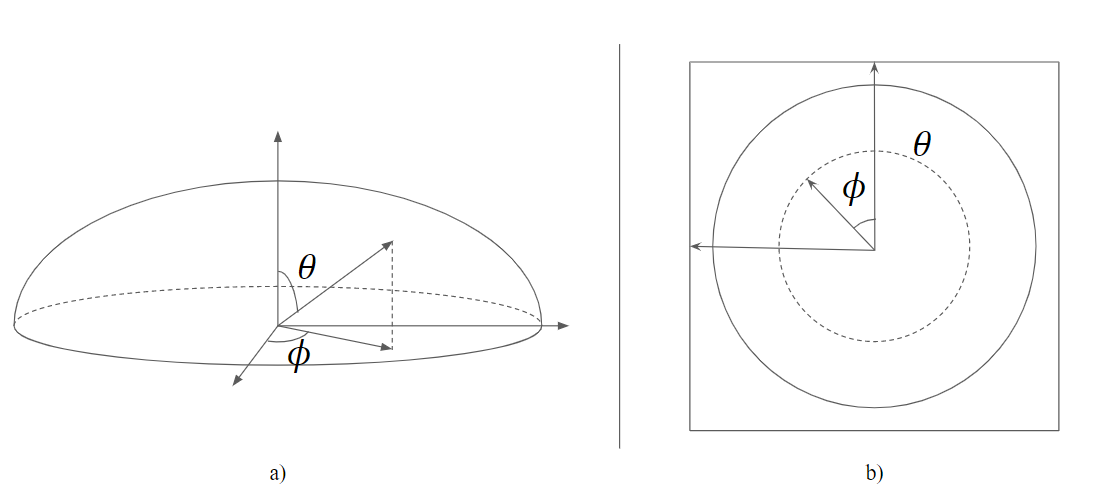
\includegraphics[width=0.95\textwidth]{coordinates.png}
\caption{\label{fig:coordinates} (a) the basic setup for the spherical coordinate system is depicted. Here, the hemisphere represents an abstraction of the cars placement with respect to the origin. (b) The corresponding texture-space coordinate. It should be noted that all points with the same $\phi, \theta$ coordinates would be assigned to the same texture coordinates.}
\end{figure}

This UV-mapping scheme is limited when the surface of the car has two points with the same $(\phi, \theta)$ coordinates but different $r$ componentes exists, they would be forced to have the same dirt texture value. If there were to arise any major issues due to this implementation choice, we would reconsider another plan in the next step.

With these implementation details in mind, similar to the previous two steps, we would train the model on a dataset where we have the ground truth. I.e. we want to render a car with a target weathering texture and use these rendered images as our training data. The main reason for taking a side-step from training on real data is largely for debugging purposees as GAN training can often be very difficult to debug. In particular, if a model fails, it is often unclear whether it's due to a mistake in the model design or a bug in the code.

\subsection{4. Training on a real dataset}

Finally, with strong evidence that the model can learn a target texture, we want to train the model on a real dataset featuring real cars on streets. Potential datasets are the KITTI Dataset (\cite{kitti}), the Berkeley Driving Dataset (\cite{bdd}) and the Cityscapes dataset (\cite{cityscapes}). We expect that real datasets will introduce artifacts and failure modes. We describe some of them as well as our general approach towards such problems in the next section.

\section{Implementation Details}

\subsection{Ray Tracer Speed}

Although the differentiable ray tracer provides very impressive results in its ability to calculate derivatives, due to the computation intensive nature of the ray tracing algorithm, the forward and backward steps of the ray tracer are admittedly quite slow with a runtime of over 8-9 seconds per iteration when rendering medium resolution images of very simple scenes on the CPU. Since the networks are expected to run for up to 10k iterations until convergence, model training turnover could become too slow as the complexity of the model and the scene increases. Should this become an issue, we would further improve the performance by using batch rendering, and parallelization over multiple GPUs, etc.

\subsection{GAN Training}

GANs are notoriously difficult to train (\cite{ganhard}). Throughout the training process, the discriminator network learns representations for a subset of features it can utilize in order to distinguish between real and generated images. In the best case, the discriminator would learn to distinguish between real and fake weathering textures on the surface of the car. The generator would be able to then utilize this fact to learn to make realistic textures that the discriminator cannot distinguish. However, since the discriminator receives very little supervision on which subset of features it should learn to identify and which to ignore, it is very prone to learn features intrinsic to rendered images instead. The discriminator learning these features would imply that it has the ability to differentiate between real and rendered images. I.e. the texture the generator produces wouldn't be able to influence the discriminator's decision since all images that use the texture would use a ray tracing step to produce an image. Below, we describe some notable discrepancies between real and rendered images that could be observed between real and rendered images that the discriminator might abuse.

\begin{enumerate}
    \item Real images have very complex backgrounds which are very difficult to emulate in a rendered scene. By masking out the background for all scenes (real and rendered), we could let the discriminator focus only on the object for which we are learning a texture map for.
    \item Reflections on specular surfaces show the complex environment they are in; something a rendered image would struggle to replicate. We could solve this issue by putting the object in an environment map which would make the specular reflections reflect a panoramic image (this is a common technique used in computer graphics literature).
\end{enumerate}

Similar to points in the list above, we could expect other artifacts to cause hiccups in the training process which we cannot predict until we observe individual instances of such issues. Regardless, we will attempt to apply simple tricks such as proposed above to combat every issue individually on a case by case basis.

\section{Expected Contributions}

The contributions this thesis would provide are threefold:

\begin{enumerate}
    \item We would have a robust model by which the Toyotacity project's simulated urban environment would have more visual diversity and a more realistic look. Generating datasets with different texture configurations would be possible for a fraction of the effort compared to any manual alternatives.
    \item Provide feedback on the current implementation and interface for the pyredner python package which is used to interface with the differentiable ray tracer.
    \item Present an exemplar use case of the differentiable ray tracer, which may forster future research in applications of deep learning techniques in computer graphics.
\end{enumerate}

\section{References}

\bibliography{bib}

\end{document}